\section{Results}\label{sec:results}
% Rubric item 4 (22 pts). Answer the research questions in Section~\ref{sec:premise}
% directly; avoid raw R(t) plots unless they make a specific point.


We now use the Rayleigh--Plesset model to examine the three questions from Section~\ref{sec:questions}. The pressure-step calculations use $\kappa=1.4$ and the water properties in Table~\ref{tab:params}. We report the first collapse minimum and the most negative wall velocity reached before that minimum. The sinusoidal calculations use $R_0=10\,\mu\mathrm{m}$; for each frequency, the amplitude is measured as half the peak-to-peak radius variation over the final 20 forcing periods after an initial transient. All results below are for the incompressible spherical-bubble model, so a predicted collapse speed above our chosen $0.1c$ limit must be interpreted cautiously.

\subsection{Q1: Effect of pressure ratio and initial bubble radius}
\label{sec:results-q1}

Figure~\ref{fig:results-q1} shows how the first collapse changes as the pressure ratio $\Pi=p_1/p_0$ increases. For every initial radius tested, the minimum radius decreases and the peak gas pressure rises sharply with $\Pi$. At $R_0=100\,\mu\mathrm{m}$, increasing $\Pi$ from 2 to 20 decreases $R_{\min}/R_0$ from about 0.704 to 0.160 and increases the peak gas pressure from about 0.438 to 222 MPa. The latter change is much larger because the polytropic relation $p_g=p_{g0}(R_0/R)^{3\kappa}$ amplifies a reduction in radius.

\begin{figure}[htbp]
\centering
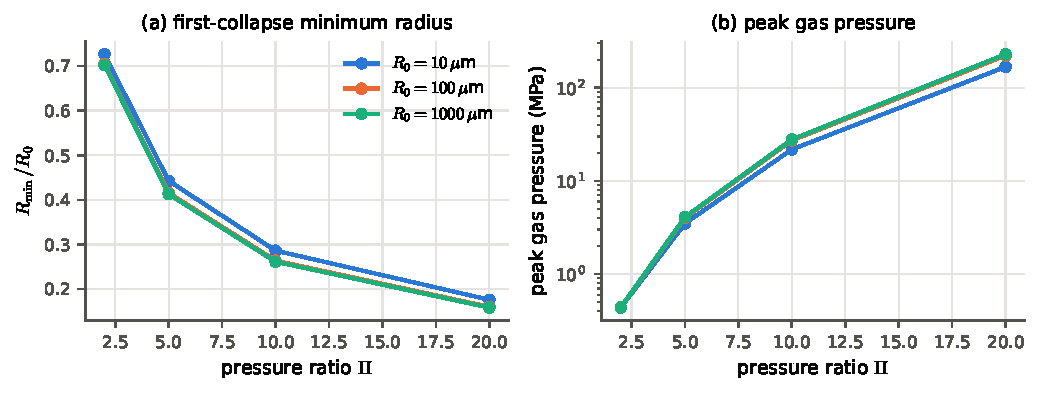
\includegraphics[width=0.96\linewidth]{q1_pressure_sweep.pdf}
\caption{First-collapse minimum radius and peak gas pressure versus the pressure ratio $\Pi$ for three initial bubble radii. The gas pressure is evaluated from the minimum radius using the polytropic model.}
\label{fig:results-q1}
\end{figure}

\begin{table}[htbp]
\centering
\small
\begin{tabular}{c|rrrr}
\hline
$\Pi$ & $R_{\min}/R_0$ & $|\dot R|_{\max}$ (m/s) & $p_{g,\max}$ (MPa) & $|\dot R|_{\max}/c$ \\
\hline
2  & 0.7043 & 5.29   & 0.438 & 0.0036 \\
5  & 0.4156 & 25.36  & 4.014 & 0.0171 \\
10 & 0.2636 & 72.18  & 27.16 & 0.0487 \\
20 & 0.1599 & 211.71 & 221.56 & 0.1429 \\
\hline
\end{tabular}
\caption{First-collapse quantities for Case~B at $R_0=100\,\mu\mathrm{m}$, $\kappa=1.4$.}
\label{tab:results-q1}
\end{table}

Bubble size also affects the collapse, but less strongly across the $10$--$1000\,\mu\mathrm{m}$ range than the pressure ratio does. For example, at $\Pi=5$, the computed minimum-radius ratios are 0.4426, 0.4156, and 0.4127 for $R_0=10$, 100, and $1000\,\mu\mathrm{m}$, respectively. The curves approach one another for larger bubbles, consistent with the dimensionless surface-tension and viscous terms becoming less important as $R_0$ increases. The gas pressure nevertheless remains crucial for stopping collapse at a finite radius; our results do not identify a universal pressure ratio beyond which gas compression can be neglected at the minimum.

The validity check is important at high pressure ratios. For $R_0=100\,\mu\mathrm{m}$ and $\Pi=20$, the predicted peak wall Mach number is about 0.143, above the $0.1$ cutoff adopted in Section~\ref{sec:ivp}. Even though the numerical integration resolves this solution, liquid compressibility may substantially affect the actual peak pressure and wall speed. We therefore treat this point as a trend predicted by the model rather than a quantitatively reliable physical value.

\subsection{Q2: Response to oscillating pressure}
\label{sec:results-q2}

Figure~\ref{fig:results-q2} compares the steady oscillation amplitude over a coarse forcing-frequency sweep at three pressure amplitudes $\varepsilon$. For the smallest forcing amplitude, $\varepsilon=0.01$, the response has a narrow maximum near $\omega/\omega_0=1$, as expected for a weakly damped oscillator. The half peak-to-peak radius variation is about $0.106R_0$ at this sampled frequency, compared with about $0.0115R_0$ at $\omega/\omega_0=0.9$. This confirms that forcing near the linear natural frequency produces a much larger response than off-resonance forcing.

\begin{figure}[htbp]
\centering
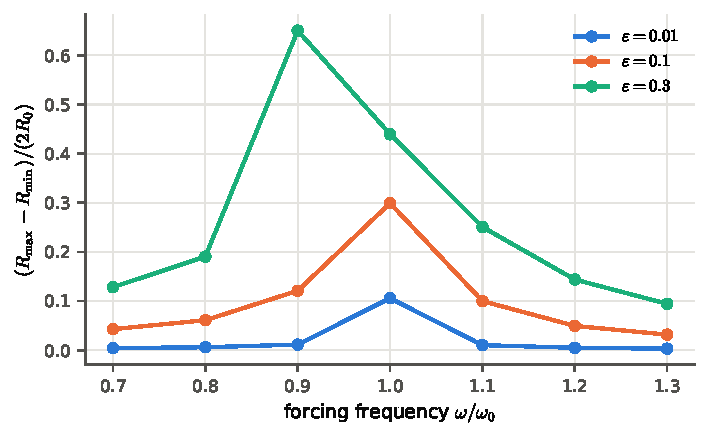
\includegraphics[width=0.78\linewidth]{q2_resonance.pdf}
\caption{Half peak-to-peak normalized radius response for Case~C at $R_0=10\,\mu\mathrm{m}$ and three forcing amplitudes. Points are sampled frequencies, not precisely located resonance peaks.}
\label{fig:results-q2}
\end{figure}

As the forcing increases, the response becomes nonlinear and asymmetric about the initial radius. At $\varepsilon=0.3$ and $\omega/\omega_0=0.9$, the simulated bubble reaches approximately $R_{\max}/R_0=1.766$ and $R_{\min}/R_0=0.465$, whereas the response at $\omega/\omega_0=1$ is smaller by the same amplitude measure. This indicates a shift in the strongest sampled response toward a frequency below the small-amplitude natural frequency. However, the current grid has a spacing of $0.1\omega_0$ and is not sufficiently fine to determine the exact peak position or the onset amplitude of violent collapse. A narrower frequency sweep around the observed maximum would be needed to quote either threshold accurately.

\subsection{Q3: Roles of surface tension and viscosity}
\label{sec:results-q3}

To isolate the forces resisting collapse, we compare the full model with calculations in which viscosity or surface tension is removed while retaining the appropriate initial equilibrium gas pressure. Figure~\ref{fig:results-q3} uses $\Pi=5$ and shows the first minimum radius for initial sizes from $1$ to $100\,\mu\mathrm{m}$.

\begin{figure}[htbp]
\centering
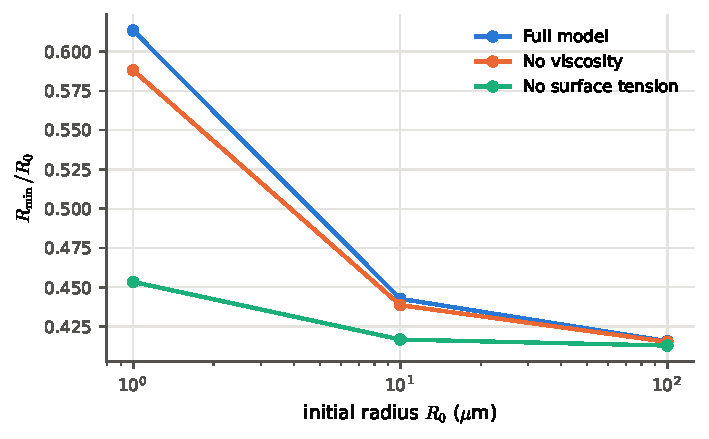
\includegraphics[width=0.78\linewidth]{q3_physics.pdf}
\caption{Effect of removing viscosity or surface tension on the first minimum radius in Case~B at $\Pi=5$, $\kappa=1.4$. The gas pressure is adjusted for the corresponding initial equilibrium condition.}
\label{fig:results-q3}
\end{figure}

At $R_0=100\,\mu\mathrm{m}$ the minimum-radius ratio changes only from 0.4156 to 0.4152 when viscosity is removed and to 0.4128 when surface tension is removed. At $R_0=1\,\mu\mathrm{m}$, these differences are much greater: the full model predicts 0.6135, removing viscosity gives 0.5881, and removing surface tension gives 0.4533. In the smaller bubble, both effects materially resist collapse, with surface tension having the larger influence under these particular conditions. The result is consistent with the dimensionless groups of Section~\ref{sec:nondim}, in which surface-tension and viscous contributions become larger as the initial radius decreases.

\subsection{Overall interpretation and limitations}
\label{sec:results-summary}

The simulations point to three conclusions. First, pressure ratio strongly controls the severity of the first collapse, and the polytropic gas law turns modest changes in minimum radius into much larger changes in peak pressure. Second, forcing close to the natural frequency produces a strong response, but the largest-response frequency can shift once the pressure oscillation is no longer small. Third, surface tension and viscosity affect micron-scale bubbles more strongly than larger ones, so changing the initial radius can alter which terms control the rebound.

These are conclusions within the spherical, incompressible Rayleigh--Plesset model. As already discussed in Section~\ref{sec:ivp}, it does not resolve shock waves, nonspherical collapse, or the thermal physics of cryogenic propellants. Furthermore, frequency maxima located from a coarse sweep should not be presented as exact resonance frequencies. Taken together with the convergence and stability checks of Section~\ref{sec:implementation}, the results demonstrate what the implemented numerical method can resolve while making clear where the underlying physical model, rather than numerical error, becomes the limiting factor.

